% !TEX root = ../MasterThesis_Onoe.tex
% 上記はただのコメントではなく親ファイルの場所を教えているので
% 消してしまうとファイルごとのタイプセットができなくなるので注意。
% 親ファイル名を変更したときはここも変更する。

\chapter{深層学習} \label{sec:Deeplearning}
本章では、本研究で提案する手法である深層学習の理論を述べる。初めに、深層学習の基礎技術であるパーセプトロンについて説明する。そしてパーセプトロンを多層にしたニューラルネットの構造と計算技術について説明する。最後に深層学習のネットワークについて、特にグラフ構造のデータを扱うグラフニューラルネットワークについて紹介する。
\section{ニューラルネットワーク}
\subsection{パーセプトロン(単層ニューラルネットワーク)}
ニューラルネットワークの基礎となるパーセプトロンは、ローゼンブラットにより1957年に考案された。パーセプトロンの基本構造は、信号を入力として受け取り論理回路を通して出力信号を出すものである。図\ref{perceptron}に最も基本的なパーセプトロンの例を示す。\\
\begin{figure}[H]
	\begin{center}
 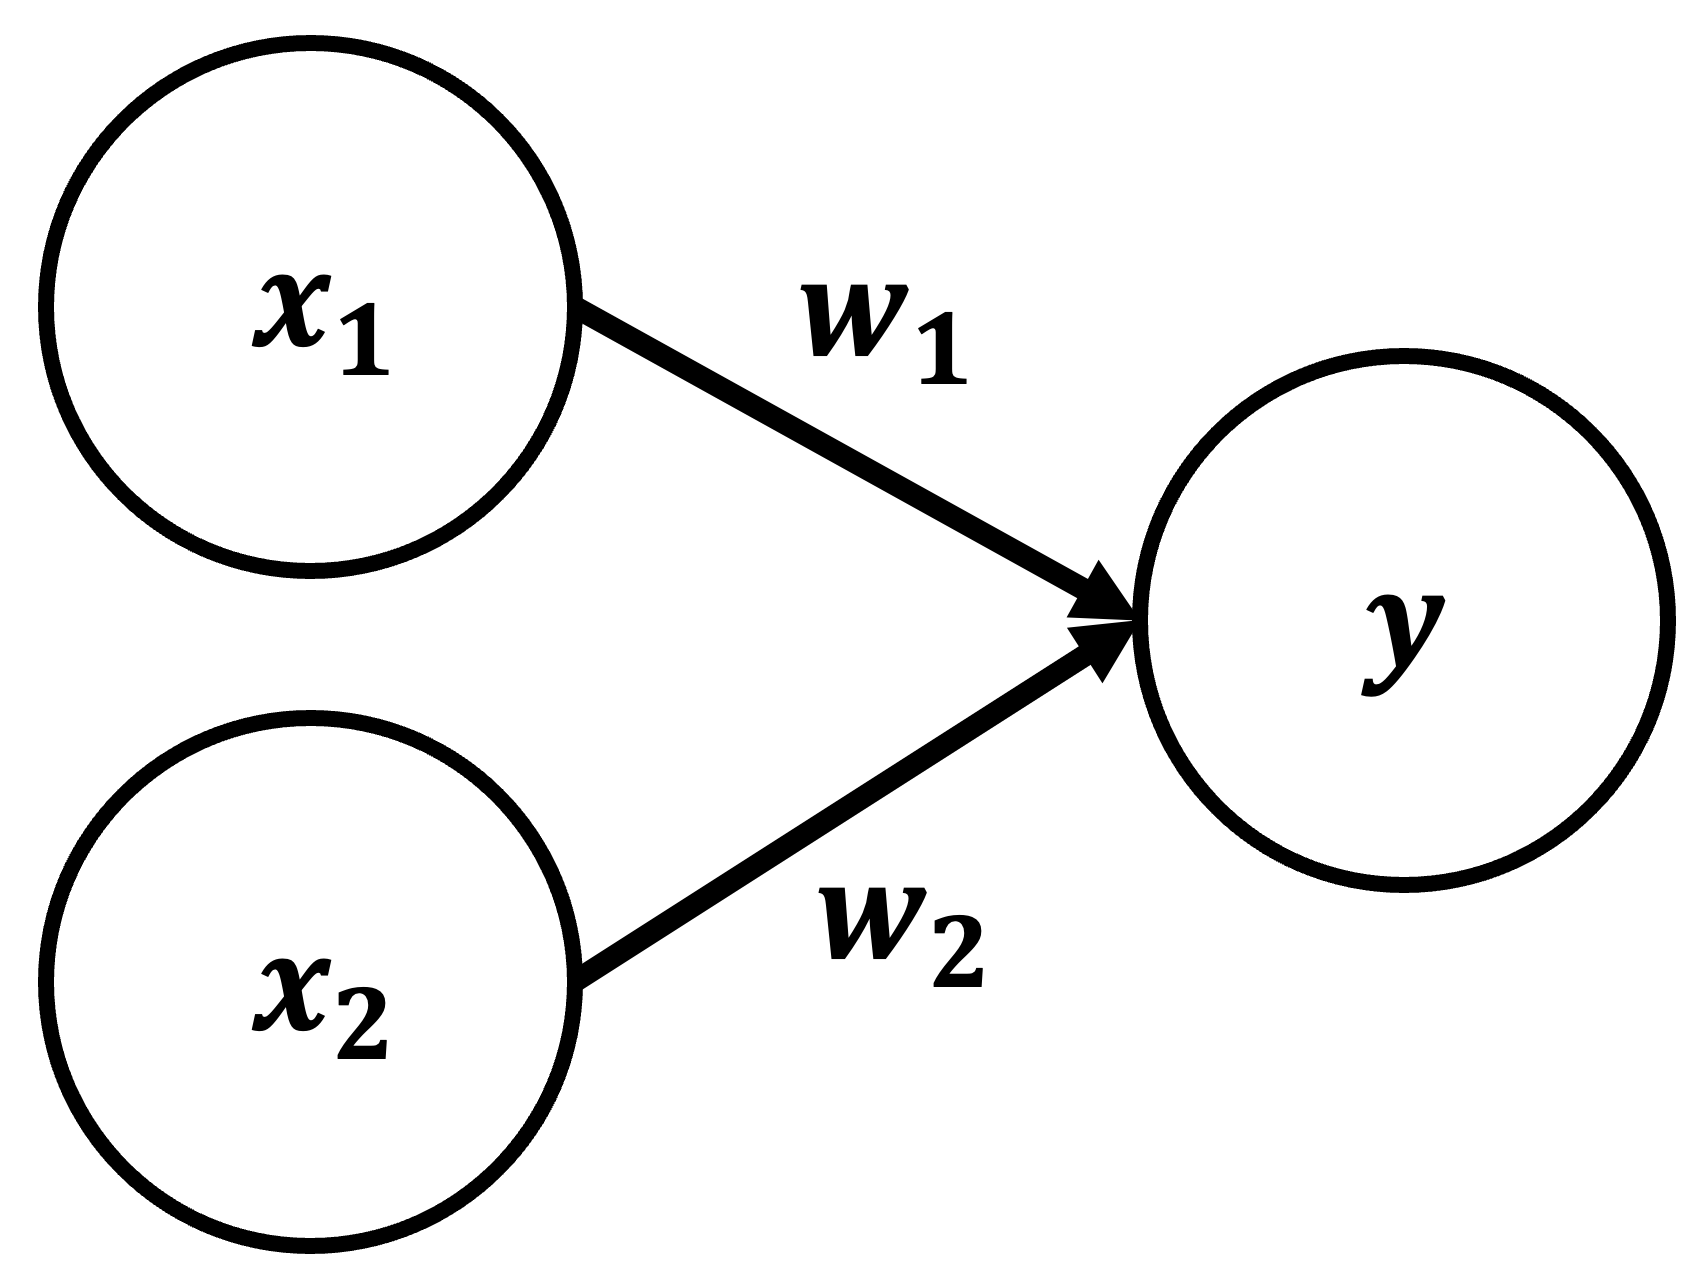
\includegraphics[keepaspectratio, scale=0.15]
 	{Figure/Deeplearning/perceptron.png}
 		\caption{パーセプトロン}
 		\label{perceptron}
	\end{center}
\end{figure}
$x_1, x_2$は入力信号、$y$が出力信号であり、$w_1,w_2$がそれぞれの入力信号にかかる重みを表す。また、図中における$\bigcirc$はノードと呼ぶ。入力信号はノードに送られる前に重みが掛けられ、出力ノードにてそれらの総和をとる。出力ノードでの演算(活性化関数)をステップ関数(階段関数)とすると、その総和が閾値$\theta$を超えている場合のみ出力信号は1を出力することになる。数式で示すと以下のようになる。\\
\begin{align}
 y =
 \begin{cases}
 0 & (w_1x_1 + w_2x_2 ) \leq \theta\\
 1 & (w_1x_1 + w_2x_2 ) > \theta \\
 \end{cases}
\end{align}
 パーセプトロンにおいて重要となるのは入力信号に対する固有の重みであり、重みは各信号の重要性を操作する要素として働く。すなわち重みが大きいほど、対応する信号の全体における重要性が高くなる。この重みを更新する操作を学習と呼び、ニューラルネットワークでは学習を繰り返すことで重みパラメータを理想とする値に近づけていく。\\
 また、入力信号が2つ以上の場合についても考えることができ、以下のような式で表される。入力信号$x = \{ x_1, x_2, \ldots x_n \}$、重みパラメータ$w = \{ w_1, w_2, \ldots w_n \}$、活性化関数(ここではステップ関数)を$h(x)$とすると、出力ベクトルyは以下のようになる。
\begin{align}
y = h(w^T x) =
 \begin{cases}
 0 & (w_1x_1 + w_2x_2 + \ldots + w_nx_n) \leq \theta\\
 1 & (w_1x_1 + w_2x_2 + \ldots + w_nx_n) > \theta \\
 \end{cases}
\end{align}
\subsection{多層パーセプトロン(多層ニューラルネットワーク)}
パーセプトロンの演算では線形領域のみしか表現できず、非線形領域においても扱えるよう入力層と出力層の間に中間層(隠れ層)を加えるニューラルネットワークに改良された。このような中間層を複数重ねたパーセプトロンを多層パーセプトロン(Multi Layer Perceptron, MLP)と呼ぶ。多層パーセプトロンの簡単な例を図\ref{mlp}に示す。\\
\begin{figure}[H]
	\begin{center}
 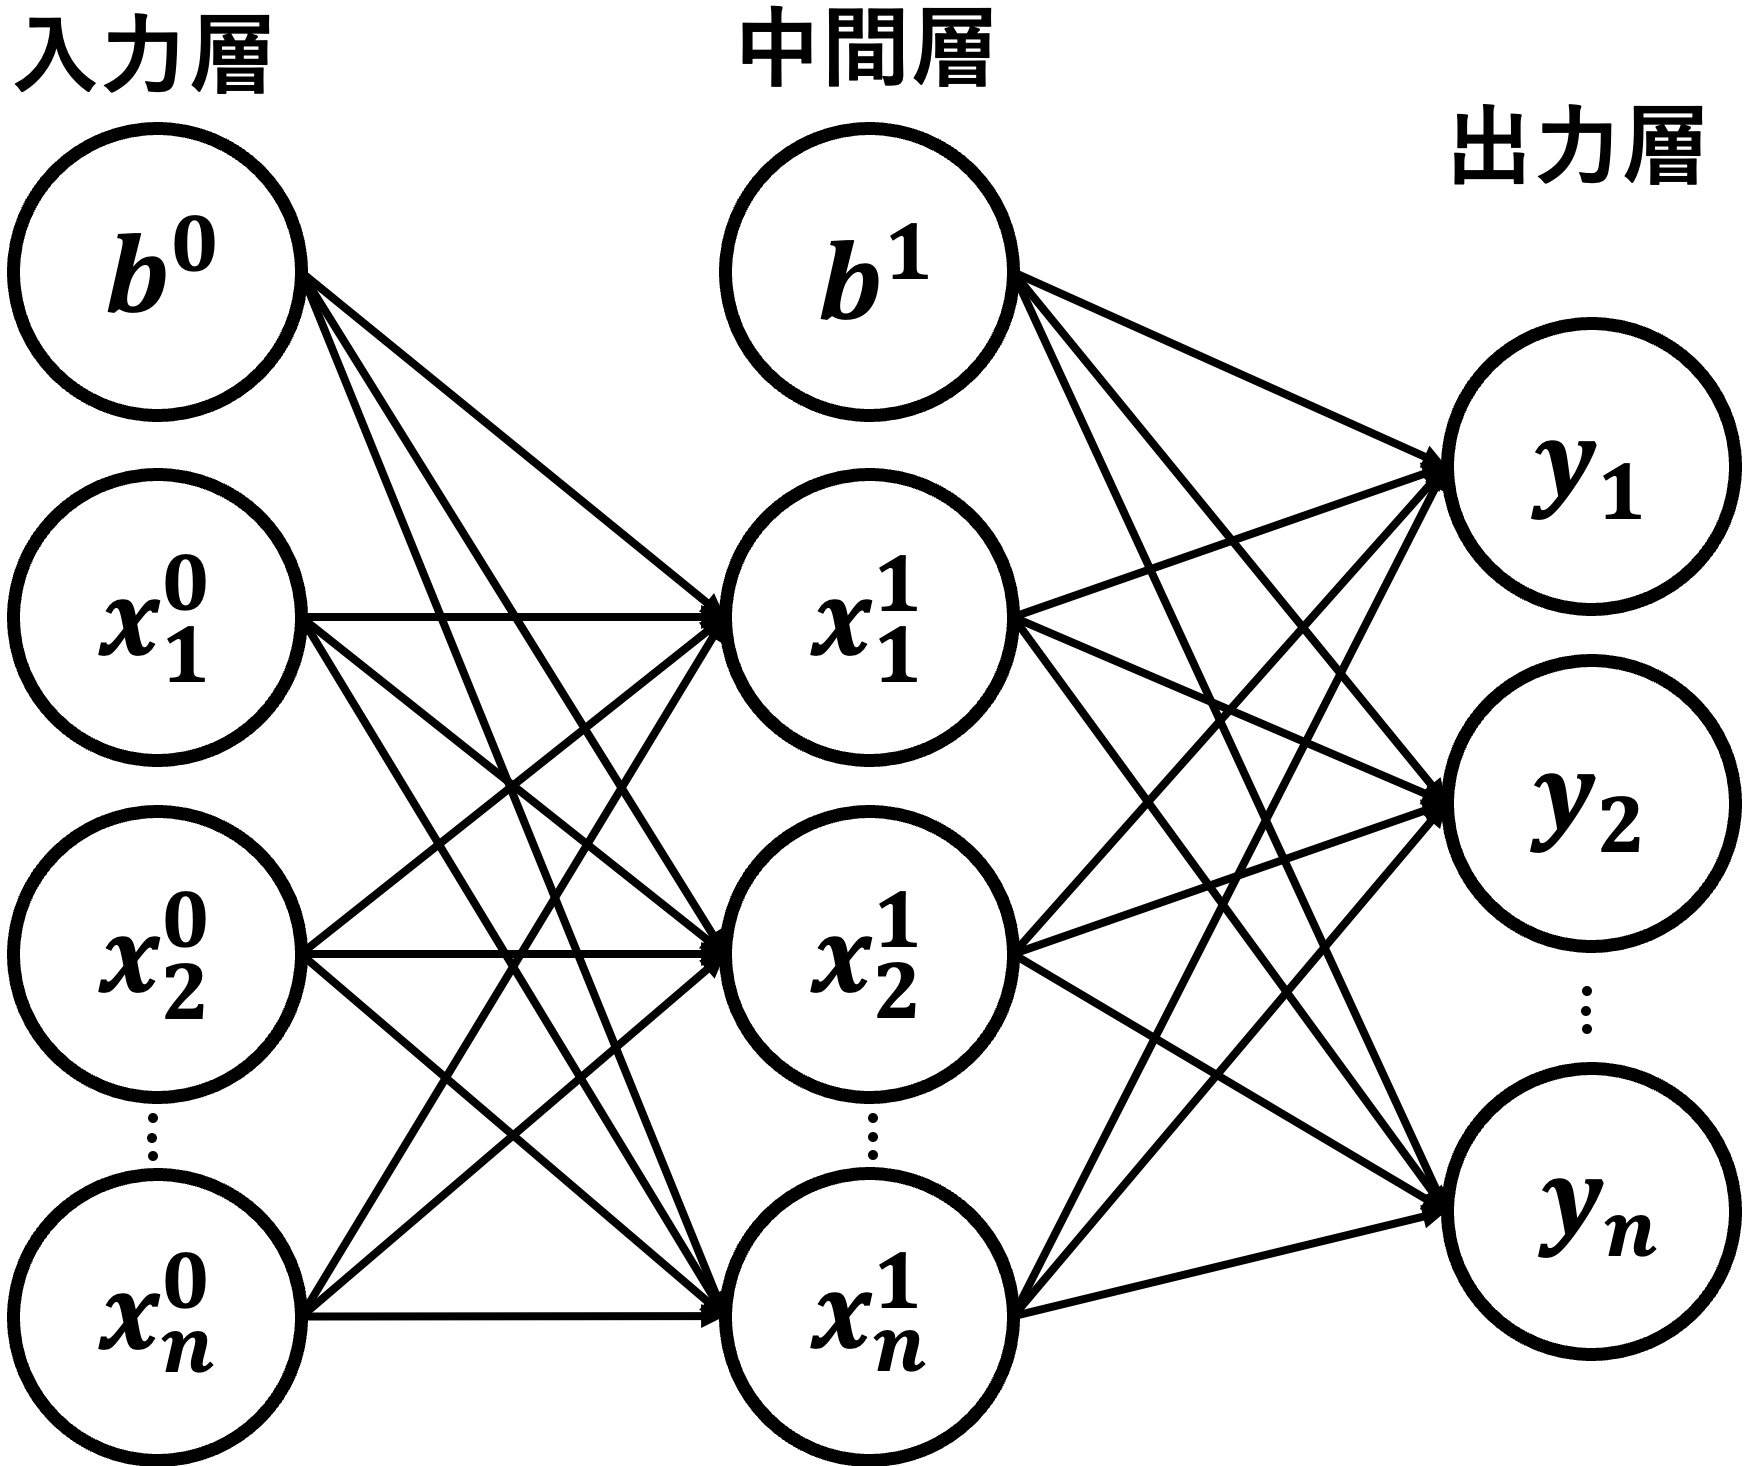
\includegraphics[keepaspectratio, scale=0.2]
 	{Figure/Deeplearning/mlp.png}
 		\caption{多層パーセプトロン(ニューラルネットワーク)}
 		\label{mlp}
	\end{center}
\end{figure}
最も左のノード列を入力層、真ん中のノード列を中間層、一番右のノード列を出力層とすると、以下のような数式で表される。入力信号$x^0 = \{ x_1^0, x_2^0, \ldots x_n^0 \}$、中間層の各ノードに入ってくる信号$x^1 = \{ x_1^1, x_2^1, \ldots x_n^1 \}$、入力層と中間層の信号にかかる重みパラメータがそれぞれ$w^0 = \{ w_1^0, w_2^0, \ldots w_n^0 \}, w^1 = \{ w_1^1, w_2^1, \ldots w_n^1 \}$、活性化関数を$h(x)$とすると、出力ベクトル$y_n$は
\begin{align}
x_1^1 = h(w_1^0 x_1^0 + w_2^0 x_2^0 + w_3^0 x_3^0 + \cdots + w_n^0 x_n^0 + b^0)\\
y_n = h(w_1^1 x_1^1 + w_2^1 x_2^1 + w_3^1 x_3^1 + \cdots + w_n^1 x_n^1 + b^1)
\end{align}
となる。ここで、$b^n$としてより学習にパラメータを加えるため、各層に実数値のバイアスを導入した。重みと信号の積の和を$a$として、上式に行列を用いると簡略に表現できる。\\
\begin{align}
\mathbf{y} = h(\mathbf{a})\\
\mathbf{a} = \mathbf{W} \mathbf{x} + \mathbf{b}
\end{align}
 以下ではニューラルネットワークの学習における、学習の仕組みや重要な技術について取り上げる。
\subsubsection{活性化関数}
活性化関数はニューラルネットワークにおける入力の重み線形和から、出力を決定するための関数である。活性化関数には主に非線形関数が用いられ、以下に主なものについて示す。
\begin{itemize}
	\item ステップ(階段)関数
		\begin{align}
			h(a) =
			\begin{cases}
			0 & (a \leq \theta)\\
			1 & (a > \theta)
			\end{cases}
		\end{align}
	\item sigmoid関数
		\begin{equation}
			h(a) = \frac{1}{1+exp(-a)}
		\end{equation}
	\item $tanh$関数
		\begin{equation}
			h(a) = tanh(a)
	\end{equation}
	\item ReLU関数(ランプ関数)
		\begin{align}
			h(a) =
			\begin{cases}
			0 & (a \leq \theta)\\
			a & (a > \theta)
			\end{cases}
		\end{align}
\end{itemize}

\subsubsection{出力層の設計}
ニューラルネットワークで扱える問題は、主に回帰問題と分類問題に分けられる。それぞれの問題によって出力層の設計が異なり、回帰問題においては恒等関数が、分類問題においてはソフトマックス関数が用いられる。恒等関数では入力された値をそのまま出力する。ソフトマックス関数は以下の式\ref{softmax}のように、0から1までの値を出力する関数であり、それぞれのカテゴリに分類される確率を表す。ここで$y_k$はニューラルネットワークの出力、$x_k$は出力層へ入ってくる信号を表す。また、出力層のノード数は問題に合わせて適宜調整する必要があり、分類問題であればカテゴリ数だけノードを設計する必要がある。
\begin{align}
y_k = \frac{exp(x_k)}{\sum_{i=1}^n exp(x_i)}
\end{align}

\subsubsection{損失関数}
先述の通り、ニューラルネットワークでは学習によって重みを更新するが、その際に学習結果を正しい答えと照らし合わせて評価し、重みを更新する。この評価関数を損失関数 (Loss function) と呼ぶ。損失関数には主に以下の2つが用いられる。
\begin{itemize}
	\item 二乗和誤差関数  (Mean Squared Error) \\
		二乗和誤差関数は、以下の式\ref{mse}で定義される関数である。ここで、$yk$はニューラルネットワークの出力、$t_k$は正解ラベルを表し、kはデータの次元数を表す。二乗和誤差関数の微分値はyの一次関数となっていることから、出力・正解ラベルが共に連続値であり恒等関数を出力層に持つ回帰問題で採用される。
		\begin{align}
			\label{mse}
			E = \frac{1}{2}\sum_k {(y_k-t_k)}^2
		\end{align}
	\item 交差エントロピー誤差 (Cross Entropy Error) 
		交差エントロピー誤差は、以下の式\ref{cee}で定義される関数である。ここで、$y_k$はニューラルネットワークの出力で、$t_k$はone-hot表現の正解ラベルを表す。交差エントロピー誤差は主にソフトマックス関数を出力層に用いる分類問題において採用される。
		\begin{align}
			\label{cee}
			E = - \sum_k t_k log(y_k)
		\end{align}
\end{itemize}

\subsubsection{誤差逆伝播法}
これまではニューラルネットワークの順方向の伝播(forward propagation)について見てきたが、出力層において学習結果と正解ラベルを比較し、逆方向に信号を伝播させ重みを更新するアルゴリズムを誤差逆伝播法 (back propagation) という。誤差逆伝播法では、次のような処理を行う。
\begin{enumerate}
	\item ニューラルネットワークにおいて順方向に学習を行い、出力層で損失関数によって正解ラベルとの誤差を求める。
	\item 誤差から各出力層ノードについて期待される出力と重要度、誤差を計算する。これを局所誤差という。
	\item 特に重要度の高い前層の入力が、局所誤差に影響を及ぼしているとして重みを調整する。
	\item さらに前層へと処理を繰り返す。
\end{enumerate}
\subsubsection{ミニバッチ処理}
ニューラルネットワークを学習させるにあたって、データを1つ1つ学習させるわけではない。実際にはミニバッチと呼ばれる、学習データをいくつかまとめて束としたものを一度に学習させる。この束をミニバッチという。また、このミニバッチのサイズ、つまりいくつのデータをまとめて束にするかという値のことをバッチサイズという。数値計算を扱うライブラリの多くは、大きな配列の計算を効率よく処理できるよう最適化がなされており、ミニバッチによる学習を行うことで、処理時間を短縮することができる。
\subsubsection{最適化アルゴリズム}
ニューラルネットワークの学習では、損失関数の値が最小となるような最適なパラメータを探索する。しかし損失関数のパラメータ空間は非常に複雑であることから、最適化は難しい。以下では、勾配降下法をはじめとする最適化手法について述べる。また、一度の学習で更新するパラメータの度合いを学習率 (learning rate) と呼んでおり、ネットワークの重みなどのパラメータとは異なり、学習率のような人の手で設定する必要のあるパラメータをハイパーパラメータと呼ぶ。
\begin{itemize}
\item \textbf{勾配降下法}\\
現在のネットワークのパラメータの微分 (勾配) を計算し、その微分の値を手がかりにパラメータの値を徐々に更新する方法を、勾配降下法 (gradient descent method) という。勾配降下法は以下の式\ref{gd}のように表される。ここで、$\mathbf{W}$は更新する重みパラメータを、$L$は損失関数を、$\eta$は学習率を表す。
\begin{align}
 \label{gd}
 \mathbf{W} \leftarrow \mathbf{W} - \eta \frac{\partial L}{\partial \mathbf{W}}
\end{align}
 また、ミニバッチ学習を用いた勾配降下法は特に、確率的勾配降下法 (stocastic gradient descent, SGD) と呼ばれており、現在のニューラルネットワークの最適化法は主にSGDに基づいて設計されている。しかし、SDGには関数の形状が等方的でない場合、勾配の方向が最終的な最小値と異なるため探索が非効率になるという欠点があり、単純に勾配方向へ進む以外の方法としてさまざまな最適化手法が考案されている。
\item \textbf{モーメンタム}\\
モーメンタム (Momentum) は、それまでの学習における損失関数上で更新ステップの動きを考慮することでSGDの振動を抑えるアルゴリズムである。モーメンタムにおける更新方法は、物理学の速度にあたる変数$\mathbf{v}$を加え、以下の式のように表される。
\begin{align}
\mathbf{v} \leftarrow \alpha \mathbf{v} - \eta \frac{\partial L}{\partial \mathbf{W}}\\
\mathbf{W} \leftarrow \mathbf{W} + \mathbf{v}
\end{align}
上式における$\alpha \mathbf{v}$が、Uの字の斜傾を転がるボールが徐々に減速する運動のような役割を果たし、振動を抑えている。
\item \textbf{AdaGrad}\\
AdaGradでは、モーメンタムと同様にSGDの振動を抑えるが、学習率を減衰させることによってこれを達成するアルゴリズムである。AdaGradの更新方法は次のような式で表される。
\begin{align}
\mathbf{h} \leftarrow \mathbf{h} + \frac{\partial L}{\partial \mathbf{W}} \odot \frac{\partial L}{\partial \mathbf{W}} \\
\mathbf{W} \leftarrow \mathbf{W} - \eta \frac{1}{\sqrt{h}} \frac{\partial L}{\partial \mathbf{W}}
\end{align}
ここで、$\mathbf{h}$はこれまでの勾配の値を二乗和として保持する役割を持つ。そして$\eta \frac{1}{\sqrt{h}}$によって学習率のスケールを調整することができる。これによって動いた大きさに合わせてパラメータ毎に学習率の減衰を行うことができる。
\item \textbf{Adam}\\
Adamはモーメントの考えとAdaGradの考えを融合させた手法であり、モーメントの変数2つと前のステップまでの学習係数を表す変数1つの3つをハイパーパラメータにもつ。これによって効率的にパラメータ空間を探索することができる。
\end{itemize}
\subsection{ディープニューラルネットワーク}
多層ニューラルネットワークにおいて、特に図\ref{dnn}のように層の数を多数持つモデルに対しては深い(ディープな)ことからディープニューラルネットワーク(Deep Neural Network, DNN, 深層学習)と呼ぶ。ディープニューラルネットワークの演算には過去に勾配消失のような技術的課題が存在していたが、計算機性能の向上に加え以下に挙げる計算技術の工夫などによって学習が可能となった。
\begin{figure}[h]
	\begin{center}
 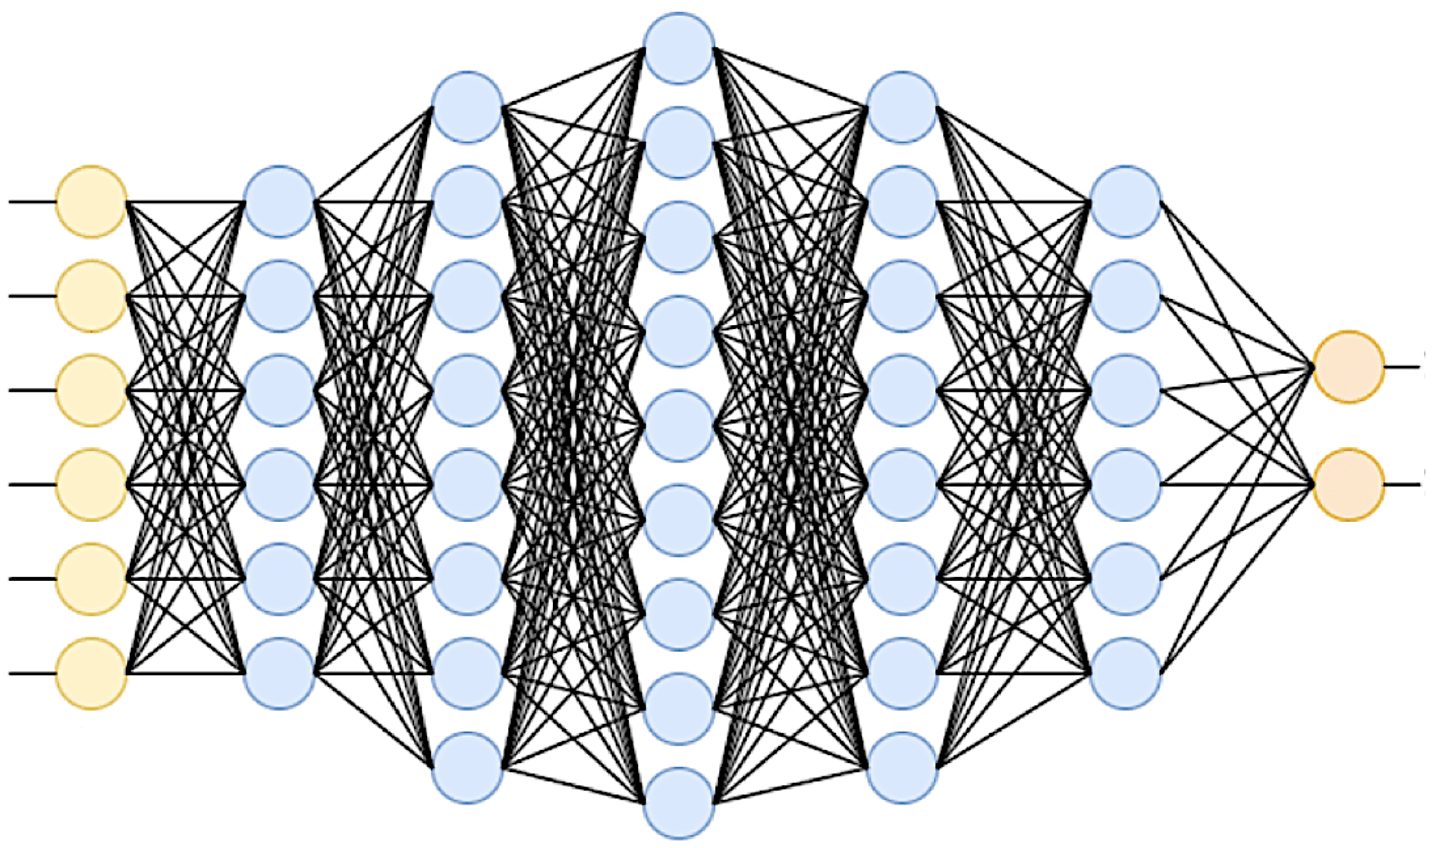
\includegraphics[keepaspectratio, scale=0.4]
 	{Figure/Deeplearning/dnn.png}
 		\caption{ディープニューラルネットワーク}
 		\label{dnn}
	\end{center}
\end{figure}
\section{グラフニューラルネットワーク}
深層学習では数値データのみでなく、画像認識や自然言語処理など様々なデータに対して目覚ましい成果を挙げている。その中で特に近年、グラフで表される構造データに対する研究が非常に盛んになっており、本研究において取り上げるグラフニューラルネットワークもその一つである。グラフ構造データとは、オブジェクトの集合(ノード)を関係(エッジ)で結んだデータのことで、ノードのみが特徴量を持つ場合と、ノードとエッジの両方が特徴量を持つ場合がある。代表的には、友人関係や論文の引用関係、化学化合物などをグラフデータとして構築することは有用であるとされており、高い表現力を持つことを強みとしている。グラフの種類は大きく分けてノードの次元が同じ同種グラフと、異なる次元のデータを扱う異種グラフの2種類に分けられる。更に、エッジが方向性を持っている有向グラフと無向グラフ、データが時系列で変化する動的グラフと変化しない静的グラフに分けられる。そしてこのようなグラフデータを扱うニューラルネットをグラフニューラルネットワーク(Graph Neural Network, GNN)という。グラフ構造や演算技術、目的とする課題によってGNNのネットワークモデルの種類は多岐にわたっており、以下では基本的なグラフでの演算や本論文に関連した幾つかの種類のモデルを取り上げる。\\
\subsection{メッセージパッシング}
GNNのアーキテクチャにおいて、グラフは集合$\mathcal{G} = (\mathcal{V}, \mathcal{E})$で構成されており、$\mathcal{V}$はノードの集合、$\mathcal{E}$はエッジの集合を表す。ニューラルネットワークの場合と同様にノードは特徴量を持っており、エッジも特徴量を持つことができる。図\ref{messagepass}にGNNにおける一般的な演算処理の流れ(メッセージパッシング)を示す。各ノードを$h_i$とすると、隣接しているノードおよびその間のエッジの特徴量を集約し、ノードを更新$h'_1$する。これによってエッジによって関連づけられたノード間で特徴量を更新していくことができる。エッジが特徴量を持つ場合は、エッジについても更新を行う。これらを数式にまとめると次のようになる。
\begin{align}
h_{(i,j)} &= f_{edge}(h_i, h_j, x_{(i, j)})\\
h'_i &= f_{node}(h_i, \sum_{j\in \mathcal{N}_i}, h_{(j, i)}, x_i)
\end{align}
ここで、$h_{(i,j)}$はエッジを、$x_i$はノードの特徴量を、$\mathcal{N}_i$は隣接しているノードの集合を表す。
\begin{figure}[H]
	\begin{center}
 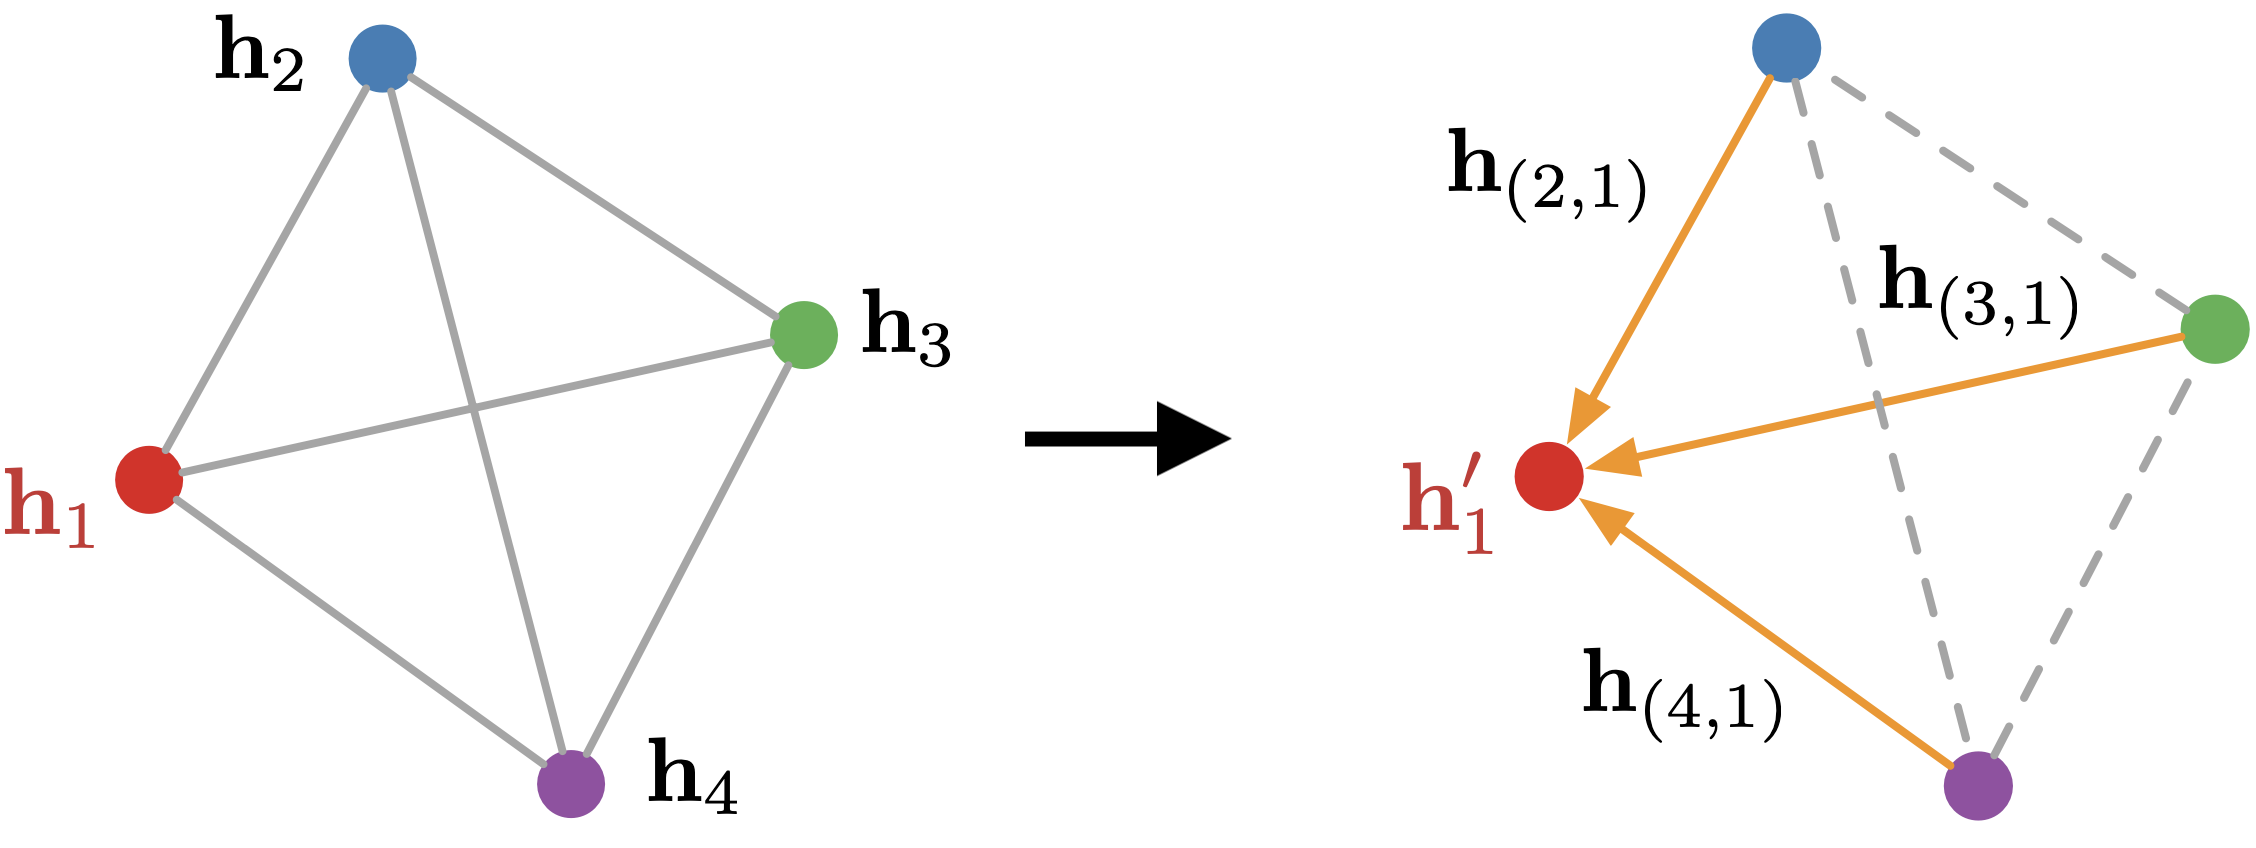
\includegraphics[keepaspectratio, scale=0.25]
 	{Figure/Deeplearning/messagepassing.png}
 		\caption{ (左) 4つのノードを持つ全結合グラフニューラルネットワーク。$h_i$はノード表現を表す。 (右) メッセージパッシングの処理。}
 		\label{messegepass}
	\end{center}
\end{figure}
\subsection{Graph Convolution Network (GCN)}
GCNとは、メッセージパッシングにおいて畳み込み(Convolution)を用いる手法である。一般的に機械学習における畳み込みは、あるフィルターを用いて対象と掛け合わせたものの和をとることで、周辺の情報を含ませることのできる処理であり、画像処理などにおいて広く用いられている。グラフの畳み込みにおいてはスペクトルによるアプローチと空間的なアプローチの2つがあり、以下ではそれぞれについて説明する。
\subsubsection{Spectral Graph Convolution}
スペクトルによる畳み込みは信号処理の考えに基づいたアプローチである。音声などの信号処理においては、関数をフーリエ変換によって周波性成分に変換し、ノイズ除去をして逆変換する。これをグラフデータに置き換えると、グラフラプラシアンの固有ベクトルが張る空間への変換・逆変換となる。グラフ信号を$\mathbf{x}$とすると、グラフフーリエ変換$\mathscr{F}(\mathbf{x})$、逆グラフフーリエ変換$\mathscr{F}^{-1}(\mathbf{x})$は次のように表される。
\begin{align}
\mathscr{F}(\mathbf{x}) &= \mathbf{U}^T\mathbf{x}\\
\mathscr{F}^{-1}(\mathbf{x}) &= \mathbf{U}\mathbf{x}
\end{align}
ここで、$\mathbf{U}$は正規化グラフラプラシアン$\mathbf{L}'$の固有ベクトル行列を表す。グラフラプラシアン$\mathbf{L}$は、グラフの隣接を表す隣接行列$\mathbf{A}$とグラフの各ノードに接続したノード数を対角成分にもつ次数行列$\mathbf{D}$を用いて、$\mathbf{L} = \mathbf{D}-  \mathbf{A}$で求められる実対称正方行列であり、正規化グラフラプラシアンは$\mathbf{L}' = \mathbf{I} - \mathbf{D}^{\frac{1}{2}} \mathbf{A} \mathbf{D}^{\frac{1}{2}}$とかける。\\
これらを用いて、グラフにおけるSpectralな畳み込み演算は次のように定義される。
\begin{align}
\mathbf{g} \star \mathbf{x} &= \mathscr{F}^{-1}(\mathscr{F}(\mathbf{g}) \odot \mathscr{F}(\mathbf{x}))\\
&= \mathbf{U}(\mathbf{U}^T \mathbf{g} \odot \mathbf{U}^T \mathbf{x})
\end{align}
$\mathbf{g} \star \mathbf{x}$は畳み込み演算を、$\mathbf{U}^T \mathbf{g}$はスペクトル領域における畳み込みのフィルターを表す。学習により更新される集合である$\mathbf{g}$に焦点を当ててより単純化すると、次のようにかくことができる。\\
\begin{align}
\mathbf{g} \star \mathbf{x} &= \mathbf{U} \mathbf{g} \mathbf{U}^T \mathbf{x}
\end{align}
 上記のように、スペクトルによる畳み込みはグラフ構造の一部が全体に影響を与えるような演算であるという特徴を持っており、さらに行列の固有値分解など計算量が多くなってしまう欠点がある。
\subsubsection{Spatial Graph Convolution}
グラフデータにおける畳み込みは空間的なメッセージパッシングの考えに基づいており、グラフ内の1つのノードが持っている特徴量に、隣接関係にあるノードの特徴量に重みをかけたものを加えていく。これによりノード自体の特徴量に加え、隣接関係や隣接ノードの特徴量の情報などを含んだ演算を行うことができる。メッセージパッシングにおける工夫に応じて様々な畳み込みのモデルが提案されているが、以下では最も一般的なモデルであるGraphSAGEについて述べる。\\
 GraphSAGE(Graph SAmple and aggreGatE)では、隣接から特徴量をサンプリングして集約することで自身のノードを更新する。
\subsection{Graph Attention Network (GAT)}

\subsection{グラフニューラルネットワークの応用}